\documentclass[12pt]{book}
\usepackage{fontspec}
\setmainfont{TeX Gyre Pagella}
\usepackage[paperwidth=8in,paperheight=8in,margin=0.6in]{geometry}
\usepackage{xcolor}
\usepackage{amssymb}
\usepackage{tikz}
\usetikzlibrary{arrows.meta}
\pagestyle{empty}
\setlength{\parindent}{0pt}

\newcommand{\artnote}[1]{{\color{gray!70}\small\itshape [Illustration: #1]}\par\vspace{0.3in}}
\newcommand{\bigline}[1]{{\Huge #1}\par}
\newcommand{\pagenum}[1]{\vfill{\color{gray!50}\footnotesize #1}}
\newcommand{\sprollpage}{\newpage\vspace*{0.4in}}

\begin{document}

\thispagestyle{empty}
\begin{center}
\vspace*{1.1in}
{\Huge \textbf{SPROLL 07}}\\[0.4in]
{\huge \textbf{Same Picture, Different Story}}\\[0.5in]
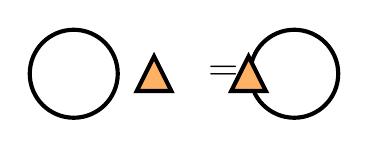
\begin{tikzpicture}
\draw[line width=1.5pt] (-1.4,0) circle (0.22in);
\draw[fill=orange!60, line width=1.5pt] (-0.6,-0.22) -- (-0.38,0.22) -- (-0.16,-0.22) -- cycle;
\node at (0.5,0) {\Large =};
\draw[line width=1.5pt] (1.4,0) circle (0.22in);
\draw[fill=orange!60, line width=1.5pt] (0.6,-0.22) -- (0.82,0.22) -- (1.04,-0.22) -- cycle;
\end{tikzpicture}
\\[0.4in]
{\large \textit{what a picture keeps, and what it lets go}}\\[0.3in]
{\small The Sproll Curriculum $\cdot$ Cycle I: Pops}
\end{center}

\sprollpage
\begin{center}
\vspace*{1.5in}
{\Large The Sproll Curriculum}\\[0.2in]
{\normalsize Cycle I --- Pops: Things, Differences, and Counting}\\[0.6in]
{\small Sproll 07 of 40 \quad $\cdot$ \quad follows Sproll 06: Look Through a Rule}
\end{center}
\pagenum{2}

\sprollpage
\begin{center}
\vspace*{0.4in}
\artnote{the two ledger strips from Sproll 02, one above the other, circle-then-triangle and triangle-then-circle}
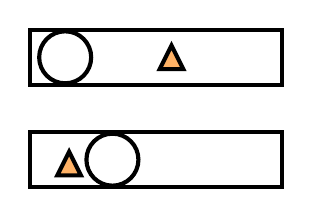
\begin{tikzpicture}
\draw[line width=1.5pt] (-1.6,0.55) rectangle (1.6,1.25);
\draw[line width=1.5pt] (-1.15,0.9) circle (0.13in);
\draw[fill=orange!60, line width=1.5pt] (0.05,0.75) -- (0.2,1.05) -- (0.35,0.75) -- cycle;
\draw[line width=1.5pt] (-1.6,-0.75) rectangle (1.6,-0.05);
\draw[fill=orange!60, line width=1.5pt] (-1.25,-0.6) -- (-1.1,-0.3) -- (-0.95,-0.6) -- cycle;
\draw[line width=1.5pt] (-0.55,-0.4) circle (0.13in);
\end{tikzpicture}
\vspace{0.25in}
\bigline{Remember these two histories?}
\end{center}
\pagenum{3}

\sprollpage
\begin{center}
\vspace*{0.6in}
\artnote{the single shared final picture from Sproll 02, circle and triangle together}
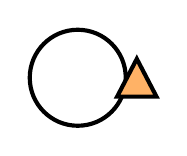
\begin{tikzpicture}
\draw[line width=1.5pt] (-0.35,0) circle (0.24in);
\draw[fill=orange!60, line width=1.5pt] (0.15,-0.24) -- (0.4,0.24) -- (0.65,-0.24) -- cycle;
\end{tikzpicture}
\vspace{0.3in}
\bigline{Rule: just show what's there.}\vspace{0.1in}
{\Large Both histories Collapse to this.}
\end{center}
\pagenum{4}

\sprollpage
\begin{center}
\vspace*{0.4in}
\artnote{the same two ledger strips again, this time drawn clearly different from each other, order visible}
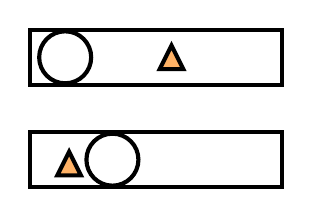
\begin{tikzpicture}
\draw[line width=1.5pt] (-1.6,0.55) rectangle (1.6,1.25);
\draw[line width=1.5pt] (-1.15,0.9) circle (0.13in);
\draw[fill=orange!60, line width=1.5pt] (0.05,0.75) -- (0.2,1.05) -- (0.35,0.75) -- cycle;
\draw[line width=1.5pt] (-1.6,-0.75) rectangle (1.6,-0.05);
\draw[fill=orange!60, line width=1.5pt] (-1.25,-0.6) -- (-1.1,-0.3) -- (-0.95,-0.6) -- cycle;
\draw[line width=1.5pt] (-0.55,-0.4) circle (0.13in);
\end{tikzpicture}
\vspace{0.25in}
\bigline{Rule: keep the order.}\vspace{0.1in}
{\Large Now they Collapse to two different things.}
\end{center}
\pagenum{5}

\sprollpage
\begin{center}
\vspace*{0.7in}
\artnote{no new image; a simple side-by-side reminder of the shared final picture and the two distinct ledger strips}
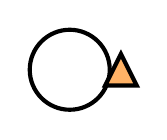
\begin{tikzpicture}
\draw[line width=1.5pt] (-0.35,0) circle (0.2in);
\draw[fill=orange!60, line width=1.5pt] (0.1,-0.2) -- (0.3,0.2) -- (0.5,-0.2) -- cycle;
\end{tikzpicture}
\vspace{0.35in}
\bigline{Same picture.}\vspace{0.1in}
{\Large Different story.}\\
{\Large It depends on the rule.}
\end{center}
\pagenum{6}

\sprollpage
\begin{center}
\vspace*{0.4in}
\artnote{the two identical-looking dots from Sproll 00, placed far apart on the page again -- one near the top left, one near the bottom right}
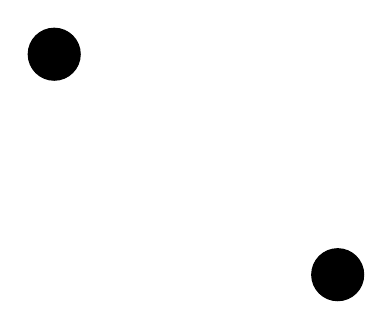
\begin{tikzpicture}
\filldraw[fill=black] (-1.8,1.4) circle (0.13in);
\filldraw[fill=black] (1.8,-1.4) circle (0.13in);
\end{tikzpicture}
\vspace{2.0in}
\bigline{Do you remember these two?}
\end{center}
\pagenum{7}

\sprollpage
\begin{center}
\vspace*{0.7in}
\artnote{the same two dots, now shown side by side and equal in size, as if compared directly}

\begin{tikzpicture}
\filldraw[fill=black] (-0.6,0) circle (0.13in);
\filldraw[fill=black] (0.6,0) circle (0.13in);
\end{tikzpicture}
\vspace{0.35in}
\bigline{Rule: ignore where things are.}\vspace{0.1in}
{\Large They Collapse to: the same.}
\end{center}
\pagenum{8}

\sprollpage
\begin{center}
\vspace*{0.4in}
\artnote{the same two dots, restored to their original far-apart positions}
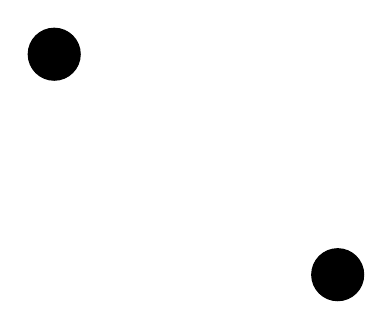
\begin{tikzpicture}
\filldraw[fill=black] (-1.8,1.4) circle (0.13in);
\filldraw[fill=black] (1.8,-1.4) circle (0.13in);
\end{tikzpicture}
\vspace{2.0in}
\bigline{Rule: keep track of where things are.}\vspace{0.1in}
{\Large They Collapse to: different.}
\end{center}
\pagenum{9}

\sprollpage
\begin{center}
\vspace*{0.8in}
\artnote{the two dots once more, small, calm, with two small labels beneath, one reading same, one reading different, neither crossed out}

\begin{tikzpicture}
\filldraw[fill=black] (-0.6,0) circle (0.13in);
\filldraw[fill=black] (0.6,0) circle (0.13in);
\end{tikzpicture}
\vspace{0.35in}
\bigline{Neither rule is the real answer.}\vspace{0.1in}
{\Large Each rule answers its own question.}
\end{center}
\pagenum{10}

\sprollpage
\begin{center}
\vspace*{0.7in}
\artnote{a small callback image: the very first page of Sproll 00, the single dot, faded and small in a corner}

\begin{tikzpicture}
\filldraw[fill=gray!35] (0,0) circle (0.12in);
\end{tikzpicture}
\vspace{0.35in}
\bigline{Sproll 00 asked: are they the same?}\vspace{0.1in}
{\Large Now you know: it depends on the rule.}
\end{center}
\pagenum{11}

\sprollpage
\begin{center}
\vspace*{0.7in}
\artnote{the boundary-scene group from Sproll 00, the small cluster inside a circle, shown once more}
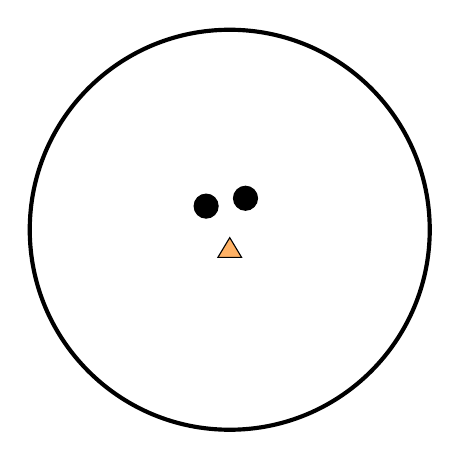
\begin{tikzpicture}
\draw[line width=1.5pt] (0,0) circle (1in);
\filldraw[fill=black] (-0.3,0.3) circle (0.06in);
\filldraw[fill=black] (0.2,0.4) circle (0.06in);
\draw[fill=orange!60] (-0.15,-0.35) -- (0,-0.1) -- (0.15,-0.35) -- cycle;
\end{tikzpicture}
\vspace{0.3in}
\bigline{The same is true here.}\vspace{0.1in}
{\Large One thing, or many, depending on your rule.}
\end{center}
\pagenum{12}

\sprollpage
\begin{center}
\vspace*{0.6in}
\artnote{a simple pair of shapes with a very deliberate, thoughtful pause -- no new content, letting the previous two answers sit side by side}

\begin{tikzpicture}
\filldraw[fill=black] (-0.6,0) circle (0.13in);
\filldraw[fill=black] (0.6,0) circle (0.13in);
\end{tikzpicture}
\vspace{0.35in}
\bigline{A picture is a kind of answer.}\vspace{0.1in}
{\Large A rule is the question it answers.}
\end{center}
\pagenum{13}

\sprollpage
\begin{center}
\vspace*{0.5in}
\artnote{two piles or boxes, unlabeled, with a small collection of shapes waiting to be sorted, as if a new kind of rule is about to be introduced}
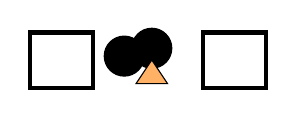
\begin{tikzpicture}
\draw[line width=1.5pt] (-1.5,-0.4) rectangle (-0.7,0.3);
\draw[line width=1.5pt] (0.7,-0.4) rectangle (1.5,0.3);
\filldraw[fill=black] (-0.3,0) circle (0.1in);
\filldraw[fill=black] (0.05,0.1) circle (0.1in);
\draw[fill=orange!60] (-0.15,-0.35) -- (0.05,-0.05) -- (0.25,-0.35) -- cycle;
\end{tikzpicture}
\vspace{0.3in}
\bigline{Some rules sort everything}\vspace{0.1in}
{\Large into just two piles: same, or not.}
\vspace{0.3in}\\
{\small \textit{--- turn the page for Sproll 08: When Are They Equal? ---}}
\end{center}
\pagenum{14}

\sprollpage
\vspace*{0.3in}
{\large \textbf{A Note for Grown-Ups}}
\vspace{0.2in}

\normalsize
This book returns to two questions this curriculum deliberately left unresolved earlier: Sproll 02's ``which happened first, if the picture can't say,'' and Sproll 00's ``are these two things the same.'' Both are now answered precisely using Collapse, introduced in Sproll 06: whether two things are ``the same'' or ``different,'' or whether an order can be recovered, is always relative to the rule used to observe them, never a fact about the underlying history in isolation.

\vspace{0.15in}
This is stated as directly as the earlier books were careful not to. The point of leaving Sproll 00 and Sproll 02 open was precisely so that this resolution would land as an answer to a question the child already holds, rather than as an isolated new fact with nothing to attach to.

\vspace{0.3in}
{\small Sproll 08: When Are They Equal? continues directly from this book's final page.}
\pagenum{15}

\end{document}
